\chapter{TLZ遷移を含むcyclic evolution}
第\ref{NT}章で,測地曲率がTwisted Landau-Zener遷移の確率に影響を及ぼすことを確認した.また,第\ref{CE}章で,Landau-Zener遷移を含むcyclic evolutionモデルにおいて,波動関数の干渉がさまざまな現象を引き起こすことを確認した.本章では,これら2つのモデルを組み合わせることによって,波動関数の干渉と測地曲率が織りなす現象が見られることを示す.

\section{整流作用を取り入れた系}

\subsection{モデルの解説}
TLZ遷移を含むcyclic evolutionに整流作用を取り入れた系におけるHamiltonianは
\begin{equation}
  \Hat{H} = \Delta_0 \sin \omega t \, \Hat{\sigma}_x +\frac{1}{4} \kappa_g \varepsilon_0^2 \cos \omega t \sin 2 \omega t \, \Hat{\sigma}_y + \varepsilon_0 \cos \omega t \, \Hat{\sigma}_z \label{TLZ_CE}
\end{equation}
である.この系における断熱エネルギーの時間変化は図\ref{fig:CEwithTLZ}のようになる.初期状態が$|2\rangle$であるとき,1番目のTLZ遷移で2つの経路に分かれる.その後,2番目以降のTLZ遷移で2つの経路の干渉が生じる.


また,Pauli行列を基底とした空間に,このHamiltonianを描写すると図\ref{fig:TLZ_CE_Pauli_1}から図\ref{fig:TLZ_CE_Pauli_3}のようになる.図\ref{fig:TLZ_CE_Pauli_1}から図\ref{fig:TLZ_CE_Pauli_3}より,この系のHamiltonianの経路は楕円を$y$軸方向にねじったような形をしている.そのため,この系はcyclic evolutionである.



\begin{figure}[htbp]
  \centering
  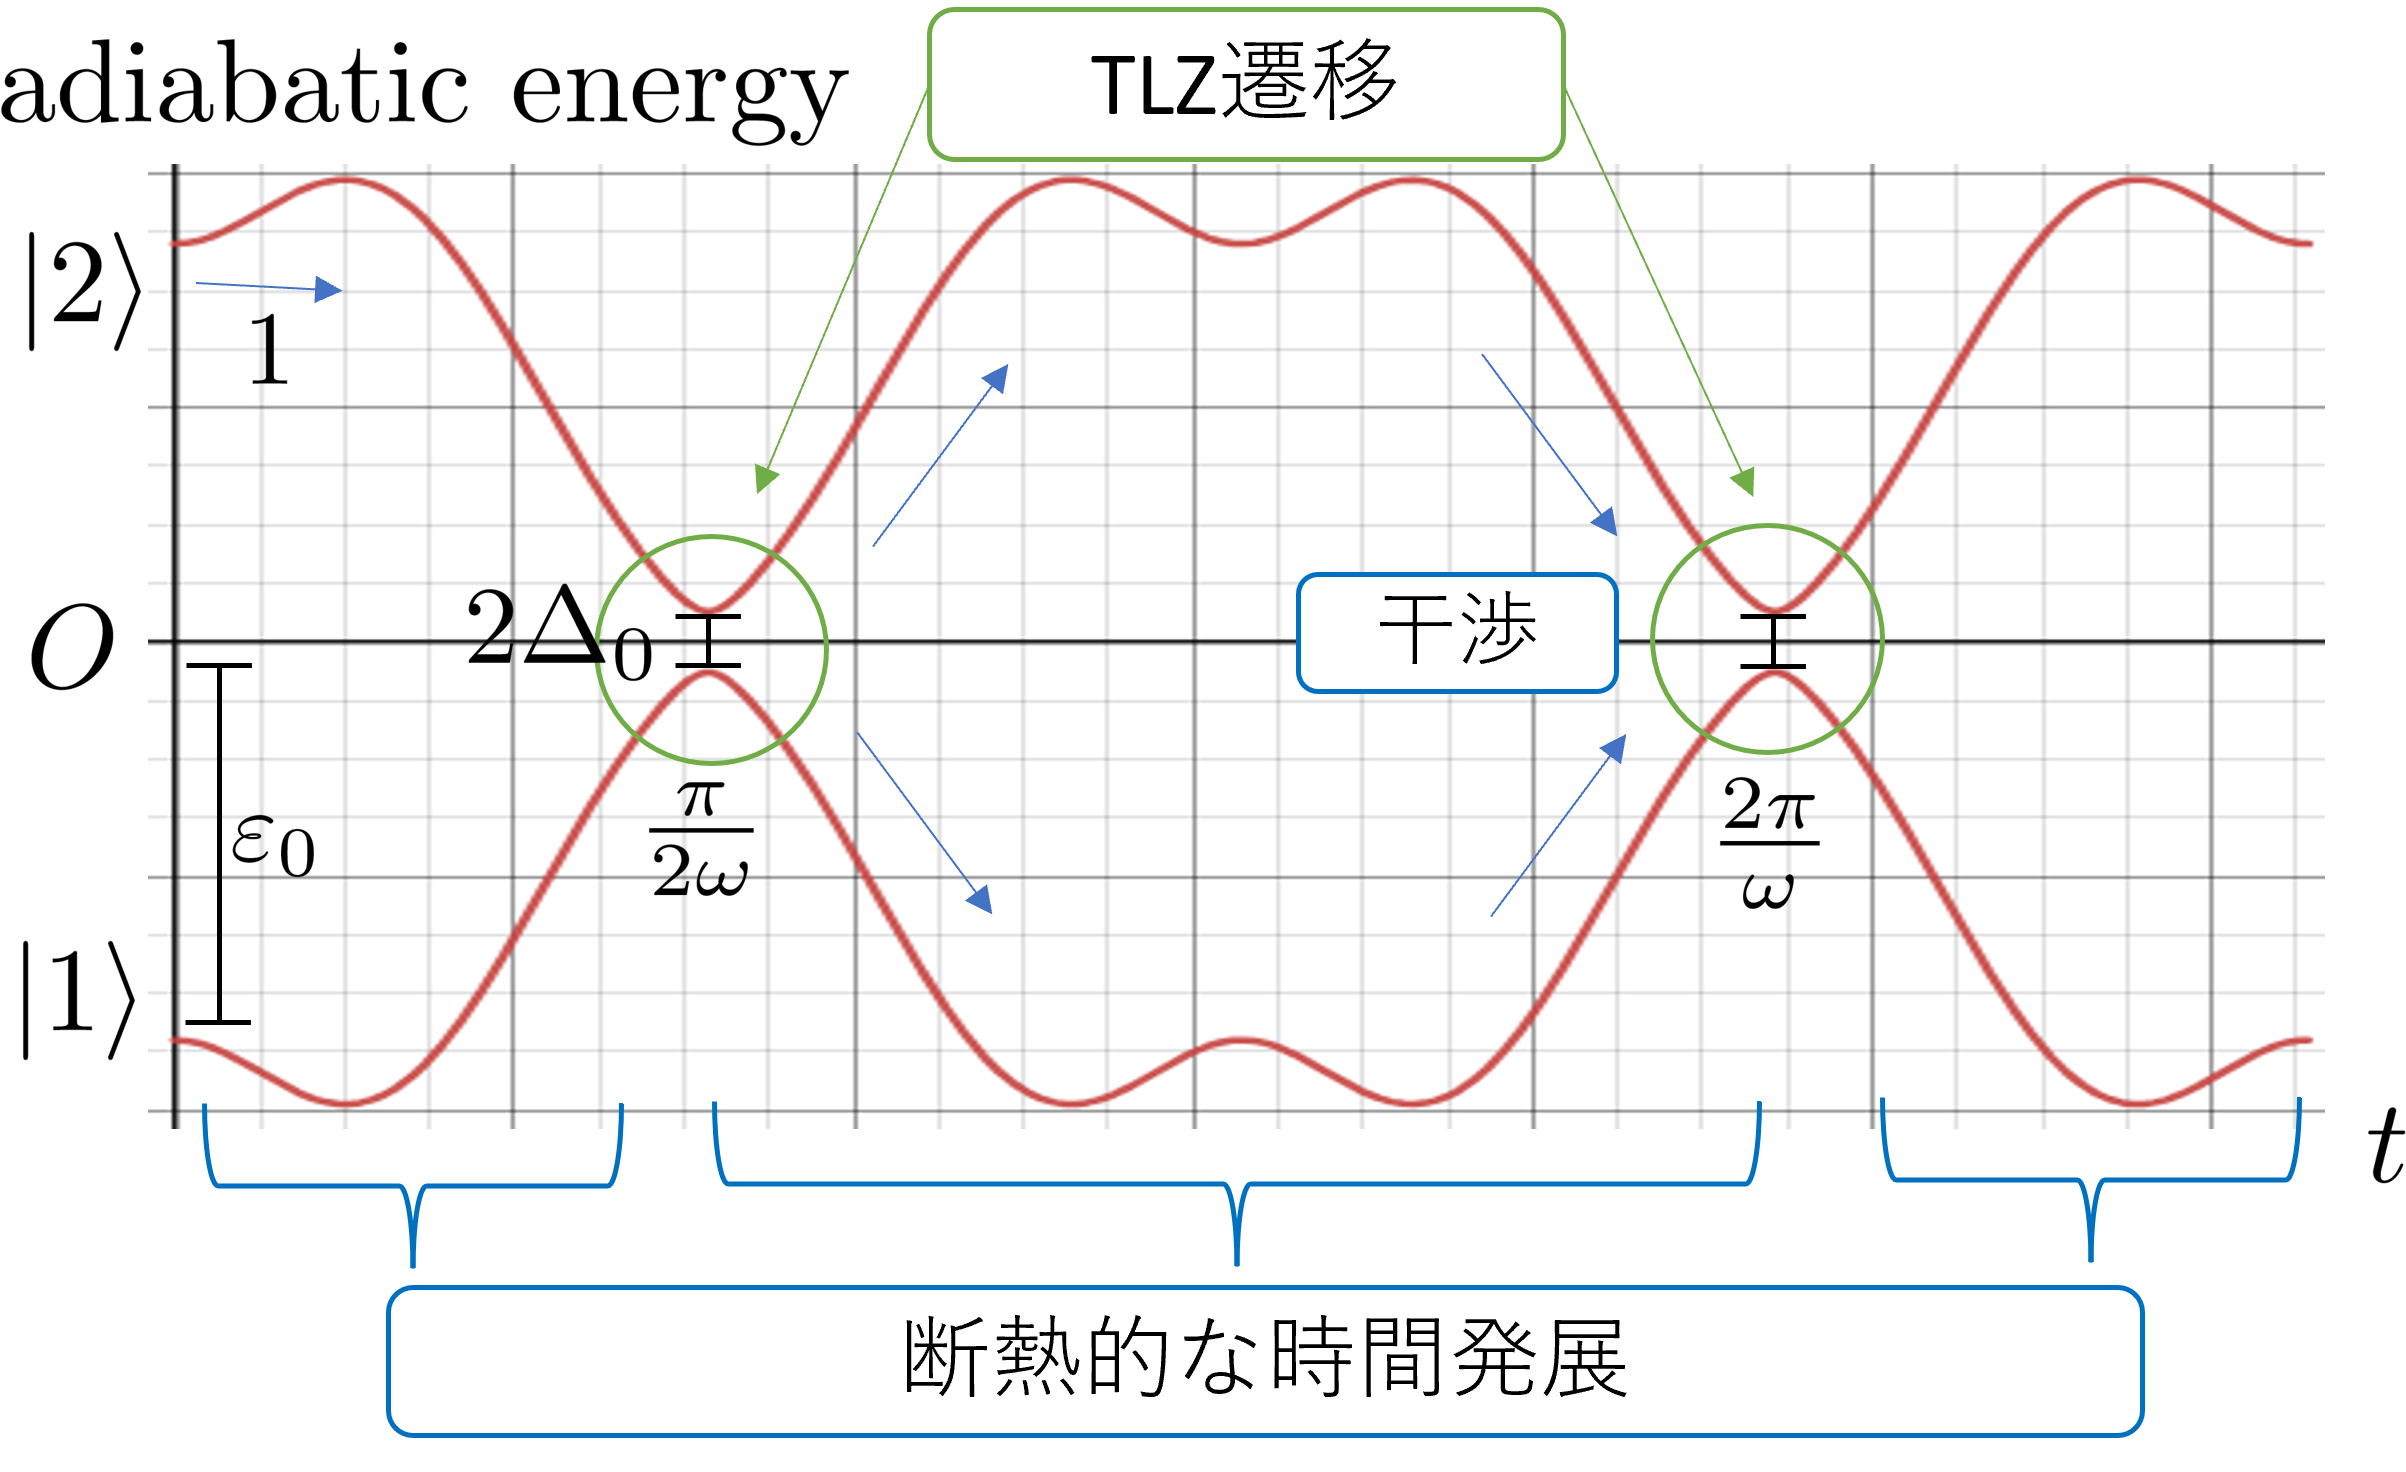
\includegraphics[scale=0.5]{figures/TLZ_CE.png}
  \caption{TLZ遷移を含むcyclic evolution(\ref{TLZ_CE})における断熱エネルギーの時間変化}
  \label{fig:CEwithTLZ}
\end{figure}

\begin{figure}[htbp]
  \centering
  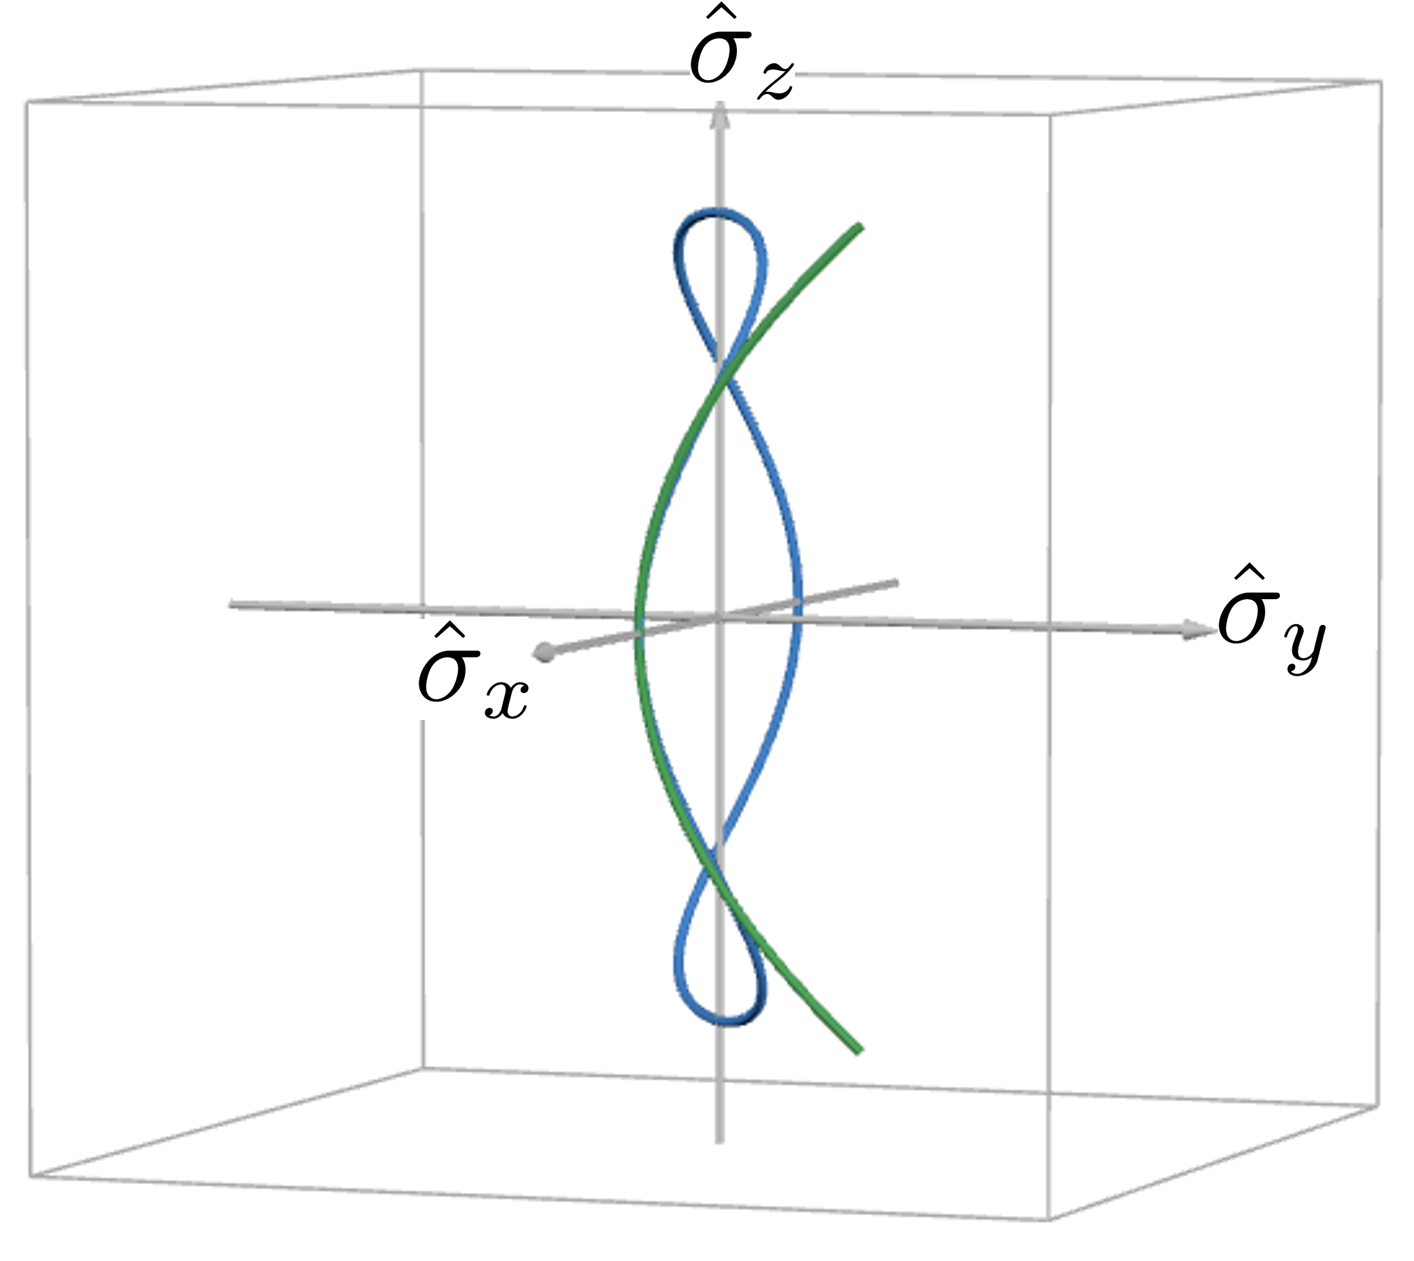
\includegraphics[scale=0.5]{figures/TLZ_CE_Pauli_1.png}
  \caption{TLZモデルを含むcyclic evolution(\ref{TLZ_CE})におけるHamiltonianの経路}
  \label{fig:TLZ_CE_Pauli_1}
\end{figure}

\begin{figure}[htbp]
  \centering
  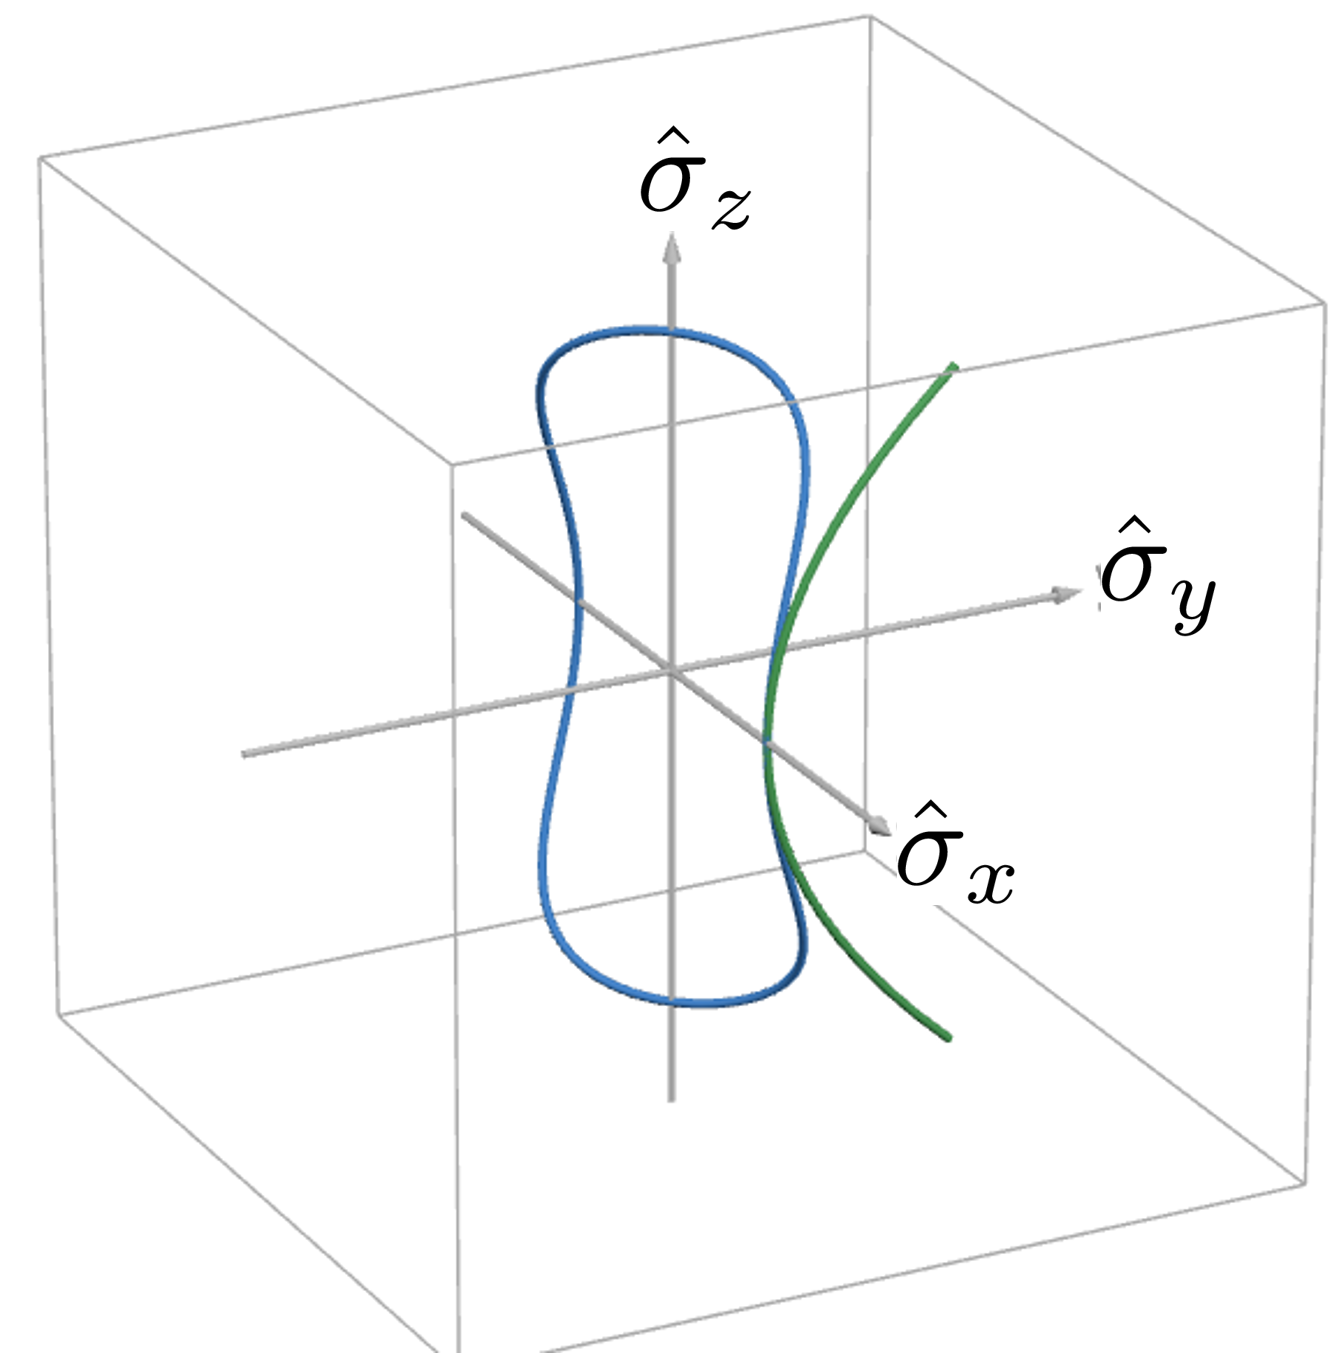
\includegraphics[scale=0.5]{figures/TLZ_CE_Pauli_2.png}
  \caption{TLZモデルを含むcyclic evolution(\ref{TLZ_CE})におけるHamiltonianの経路(別の角度からの視点)}
  \label{fig:TLZ_CE_Pauli_2}
\end{figure}

\begin{figure}[htbp]
  \centering
  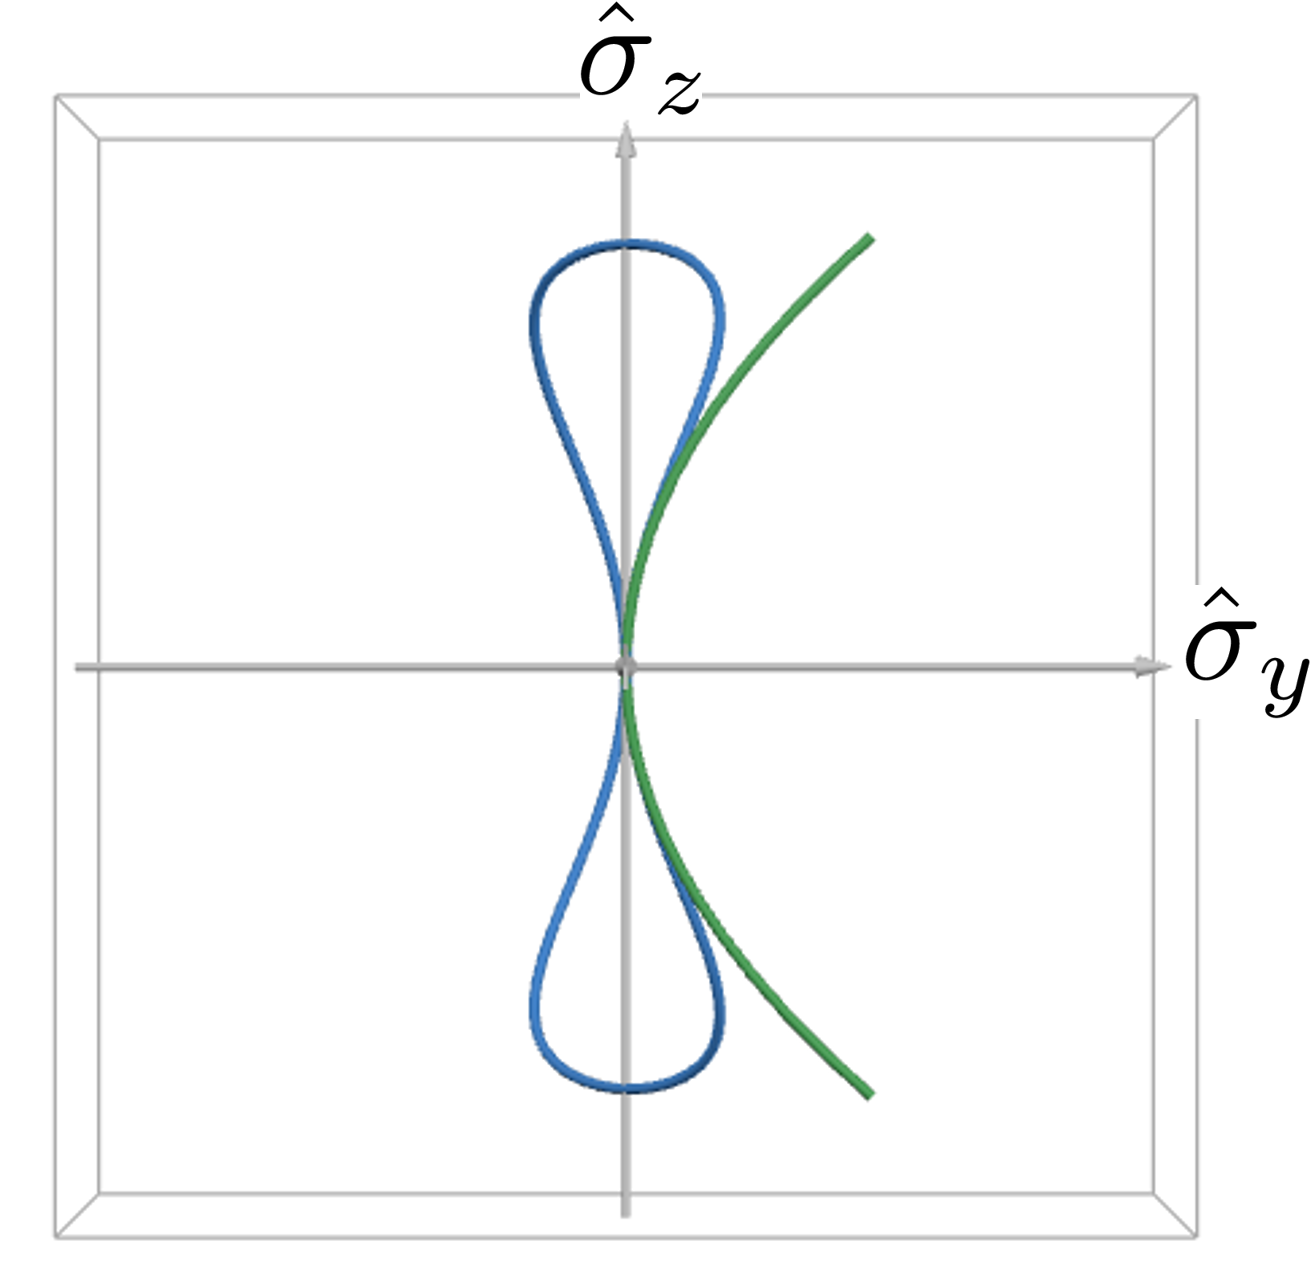
\includegraphics[scale=0.5]{figures/TLZ_CE_Pauli_5.png}
  \caption{TLZモデルを含むcyclic evolution(\ref{TLZ_CE})におけるHamiltonianの経路($x$軸視点)}
  \label{fig:TLZ_CE_Pauli_5}
\end{figure}

\begin{figure}[htbp]
  \centering
  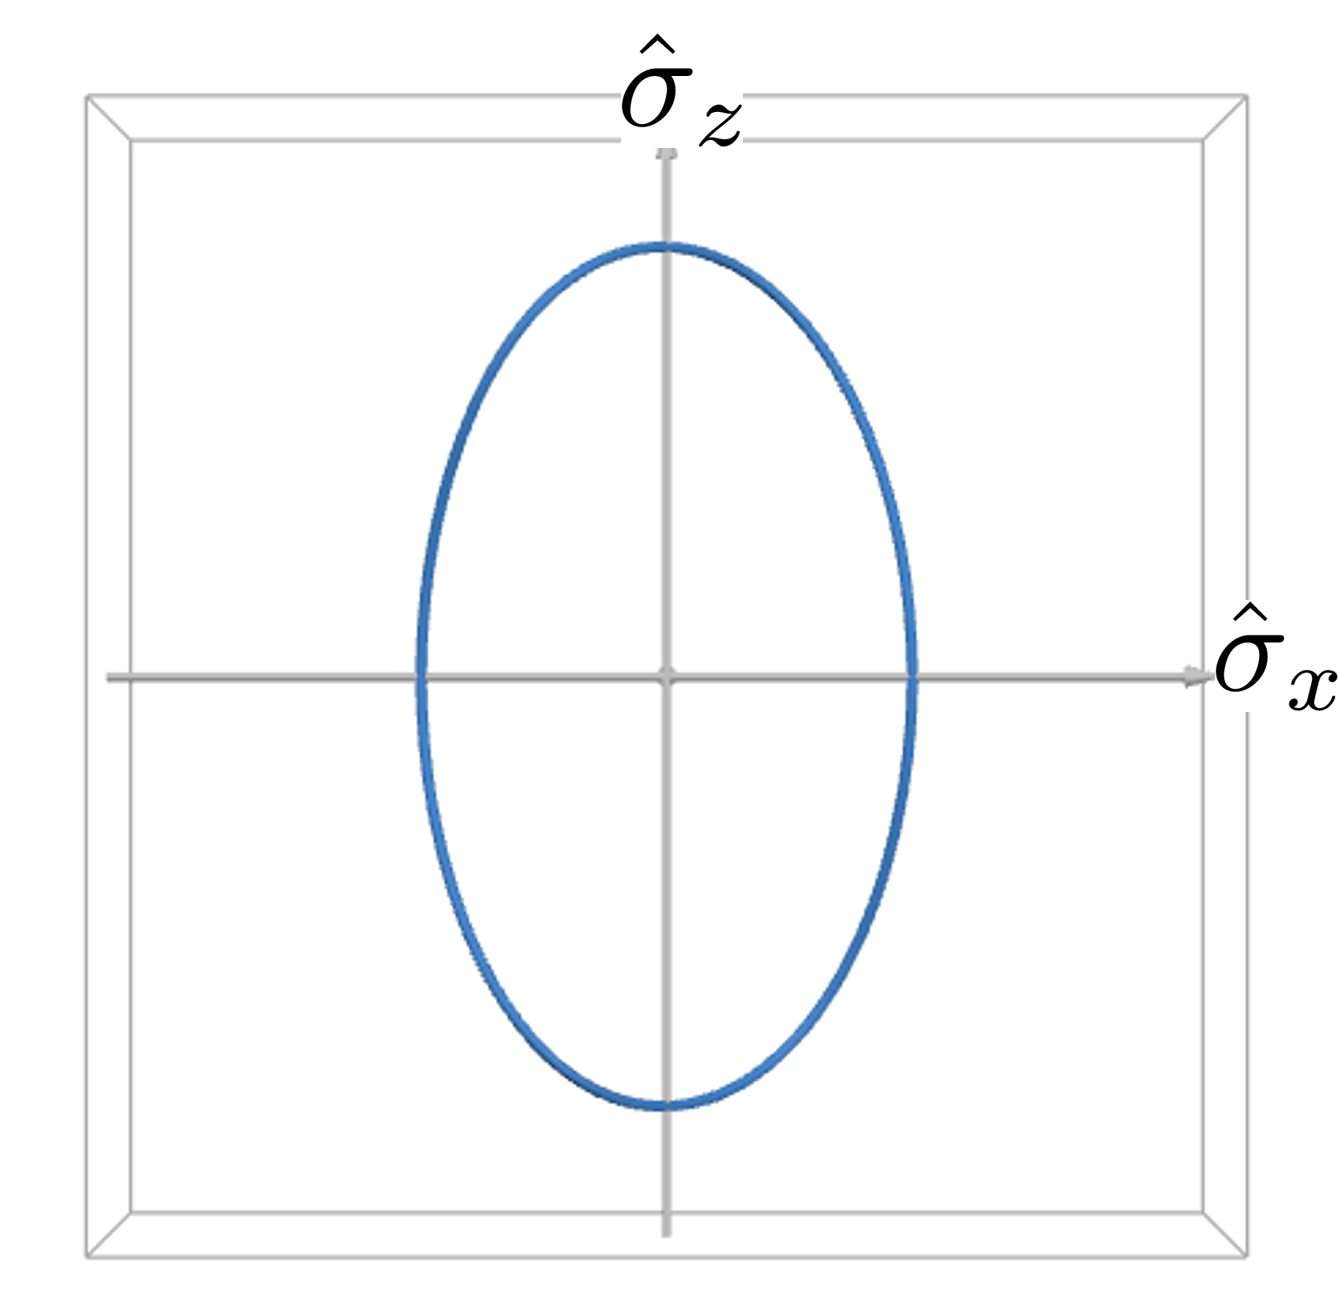
\includegraphics[scale=0.5]{figures/TLZ_CE_Pauli_4.png}
  \caption{TLZモデルを含むcyclic evolution(\ref{TLZ_CE})におけるHamiltonianの経路($y$軸視点)}
  \label{fig:TLZ_CE_Pauli_4}
\end{figure}

\begin{figure}[htbp]
  \centering
  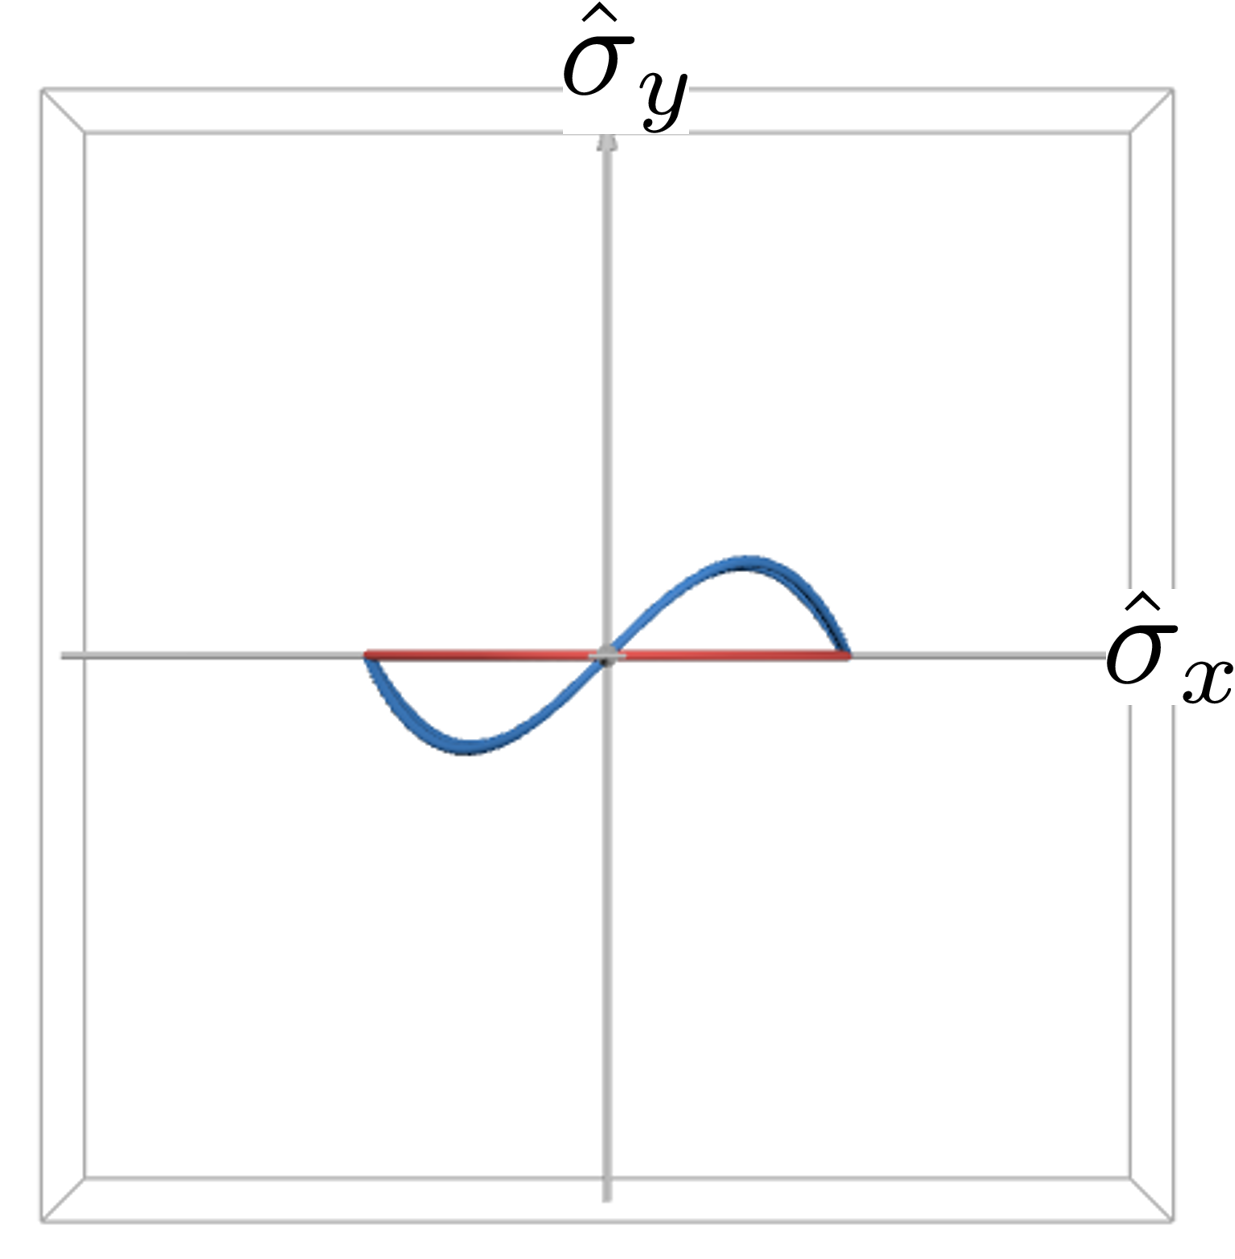
\includegraphics[scale=0.5]{figures/TLZ_CE_Pauli_3.png}
  \caption{TLZモデルを含むcyclic evolution(\ref{TLZ_CE})におけるHamiltonianの経路($z$軸視点)}
  \label{fig:TLZ_CE_Pauli_3}
\end{figure}





\subsection{数値計算の結果}
系が状態$|1\rangle$である確率($|1\rangle$ occupation probability)$P(t)$の時間変化を$\kappa_g=0.27$および$\kappa_g=0$としてそれぞれプロットすると図\ref{fig:NR_k}および図\ref{fig:NR_k=0}のようになる.


図\ref{fig:NR_k=0}では,各遷移ごとに状態の占有確率が変化する.一方,図\ref{fig:NR_k}では,2回の遷移ごとに占有確率が変化している.この現象は,完全トンネルおよび整流作用によって引き起こされると考えられる.4回目の遷移では,波動関数の干渉と測地曲率の2つの要因によって状態の占有確率が決定されていると考えられるが,詳しくはわかっていない.

\begin{figure}[htbp]
  \centering
  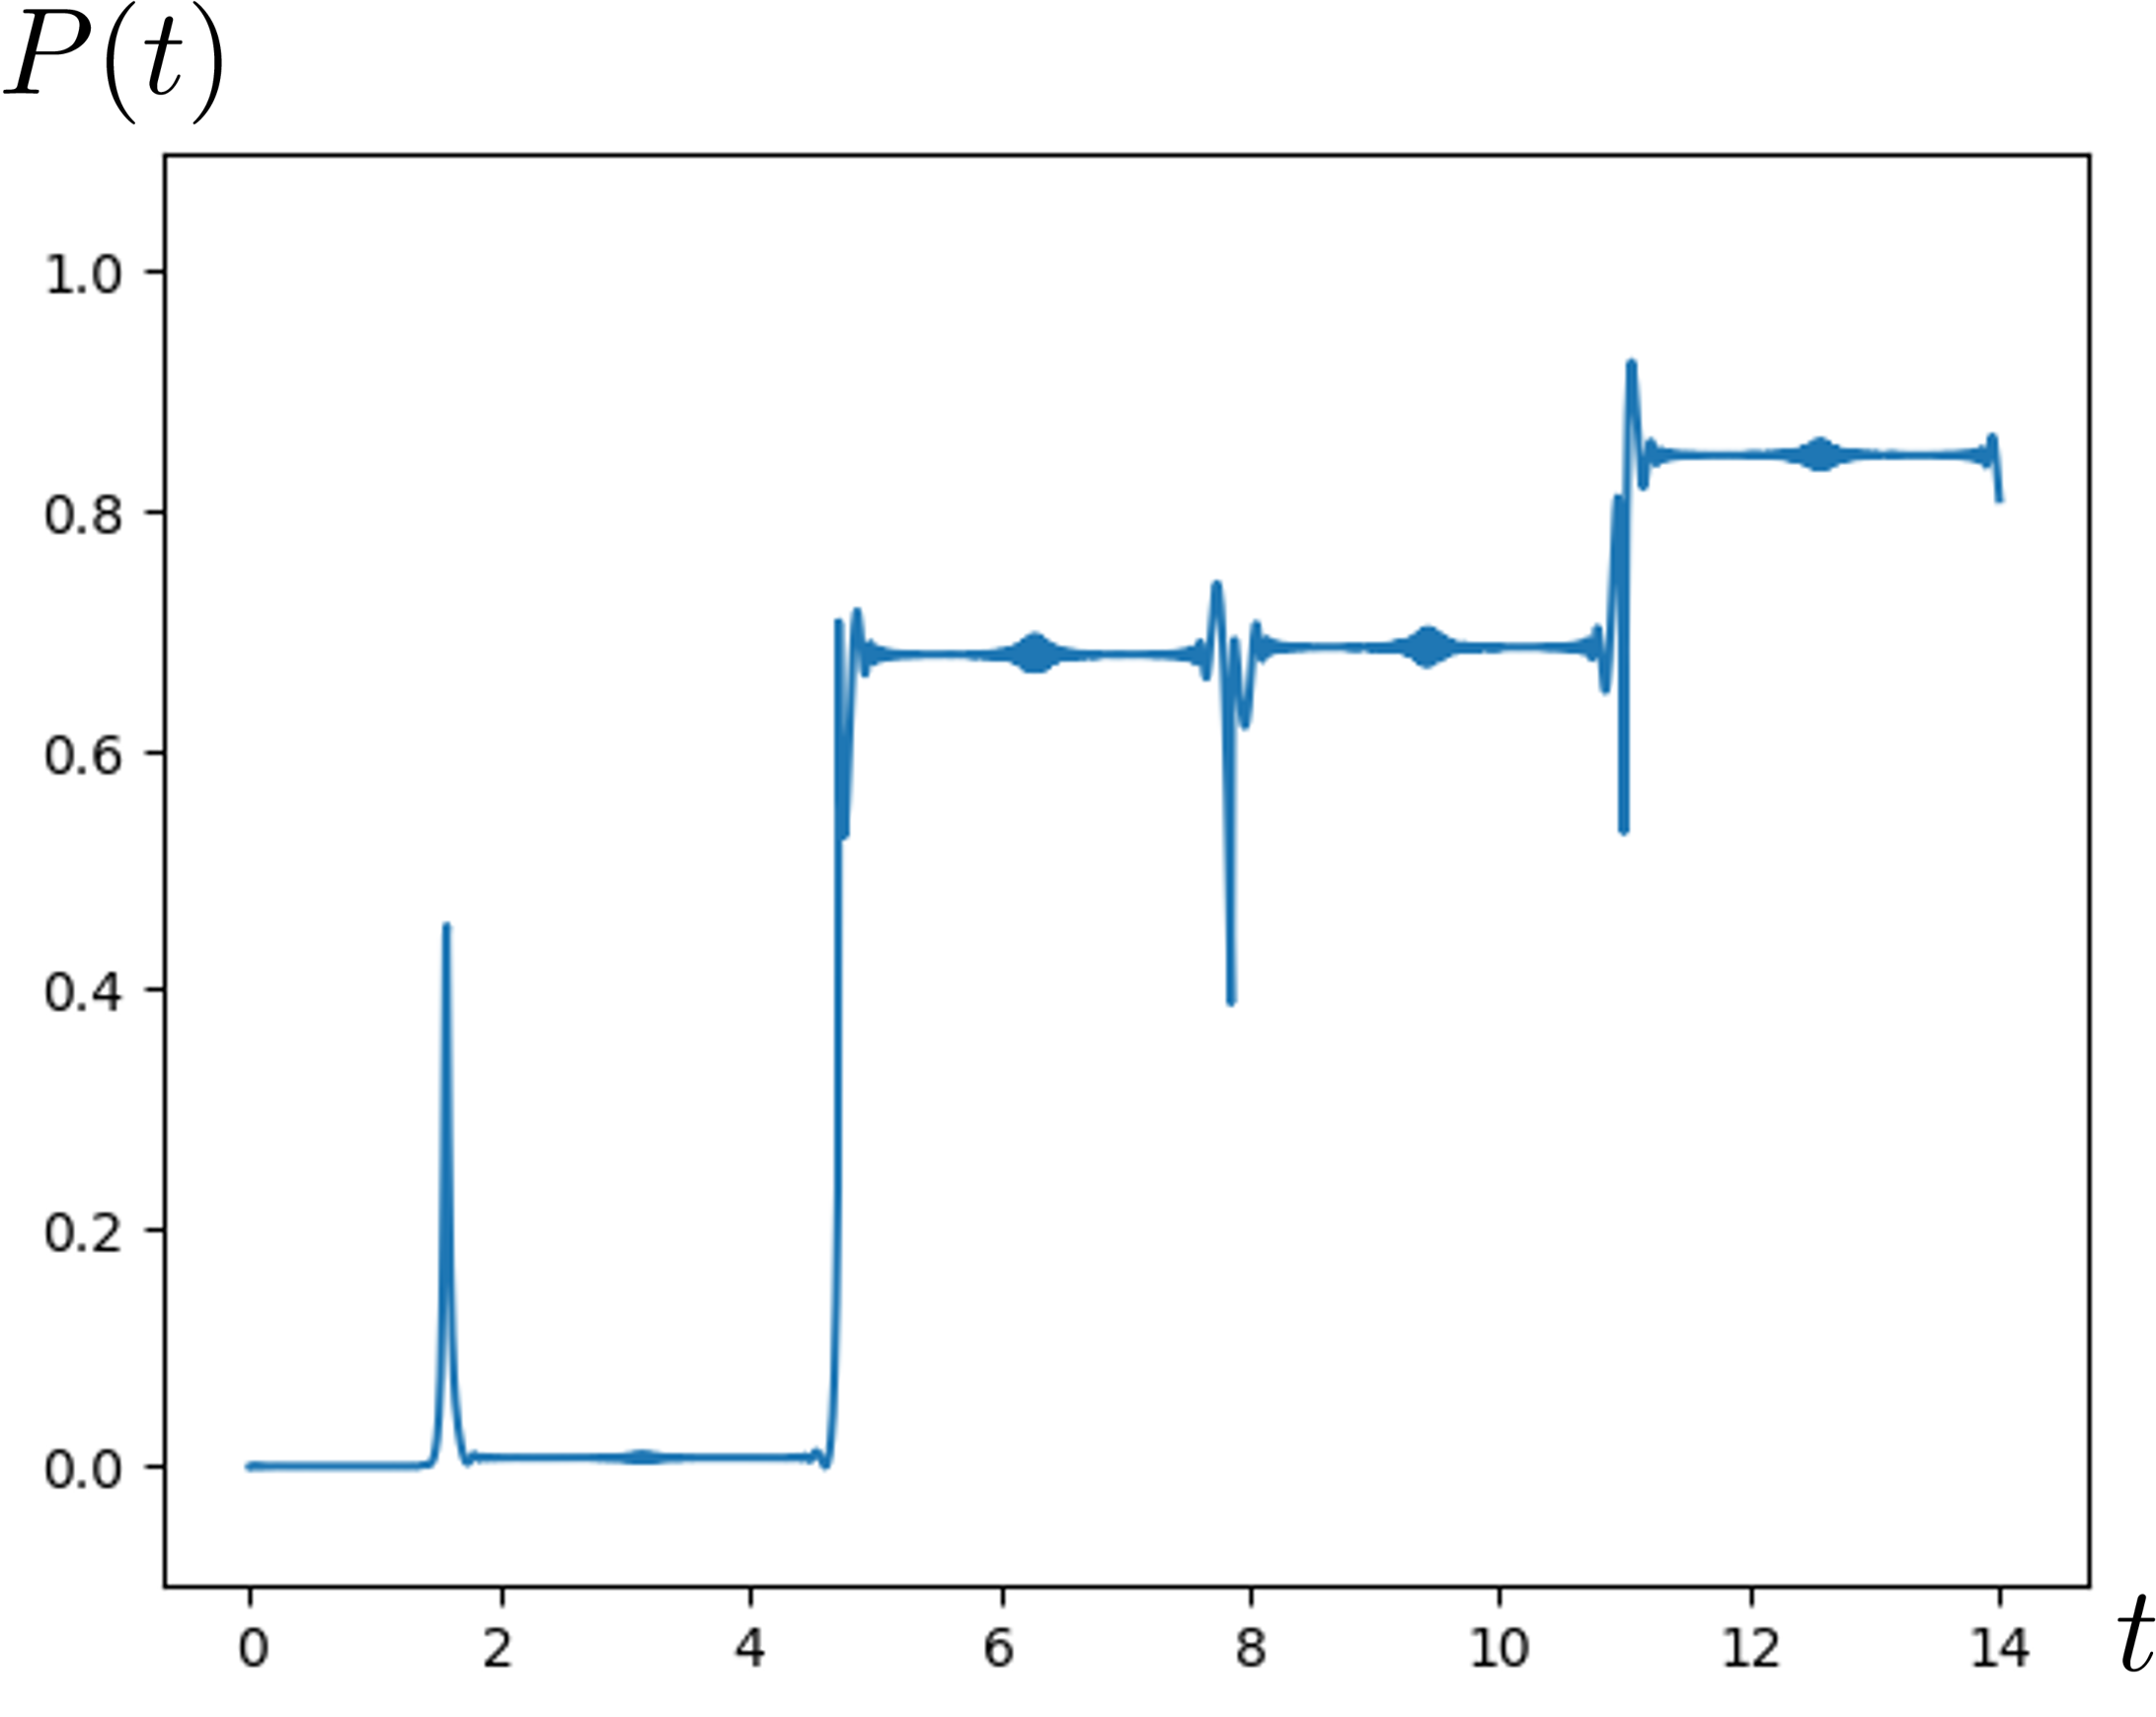
\includegraphics[scale=0.5]{figures/k_0.27.png}
  \caption{$\kappa_g=0.27$における$P(t)$の時間変化.$\varepsilon_0=90, \Delta_0 = 3, \omega=1$とした.}
  \label{fig:NR_k}
\end{figure}

\begin{figure}[htbp]
  \centering
  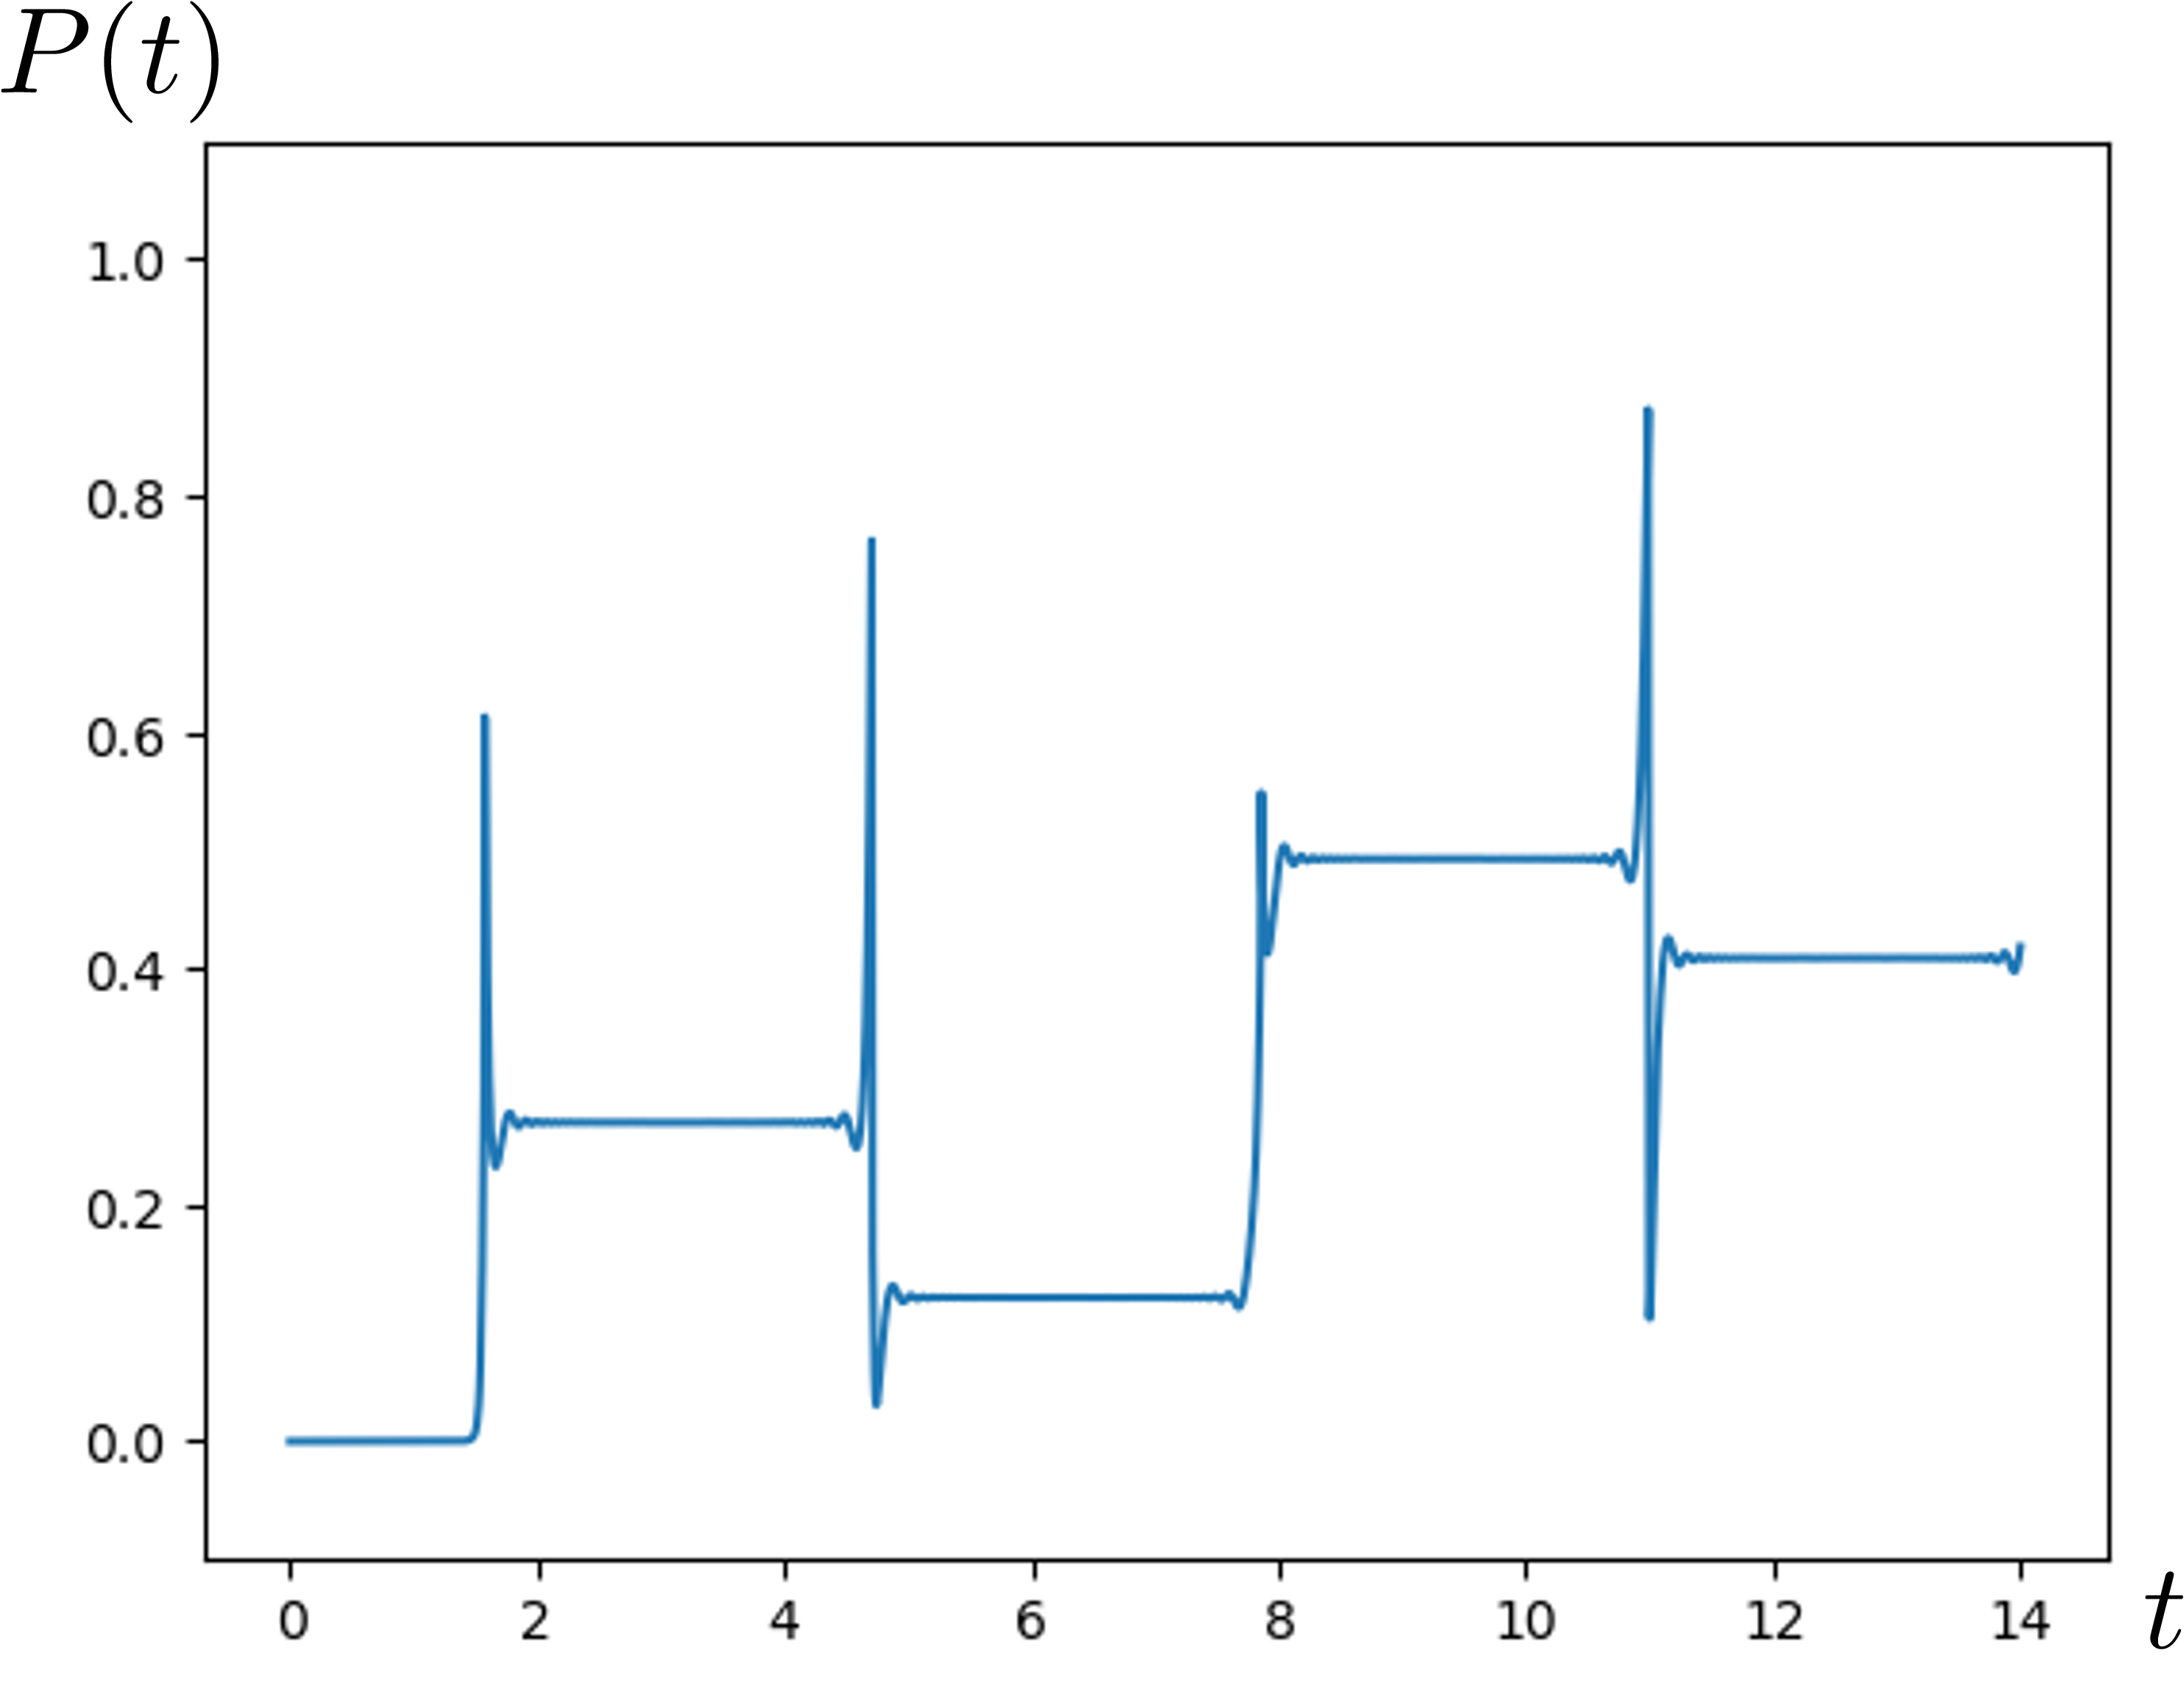
\includegraphics[scale=0.5]{figures/k_0.png}
  \caption{$\kappa_g=0$における$P(t)$の時間変化.$\varepsilon_0=90, \Delta_0 = 3, \omega=1$とした.}
  \label{fig:NR_k=0}
\end{figure}


\section{整流作用を取り入れない系}

TLZ遷移を含むcyclic evolutionで整流作用を取り入れない系のHamiltonianは
\begin{align}
  \Hat{H} = \Delta_0 \sin \omega t \, \Hat{\sigma}_x +\frac{1}{4} \kappa_g \varepsilon_0^2 \left| \cos \omega t \sin 2 \omega t \right| \, \Hat{\sigma}_y + \varepsilon_0 \cos \omega t \, \Hat{\sigma}_z \label{TLZ_CE_2}
\end{align}
である.Pauli行列を基底とした空間に,このHamiltonianを描写すると図\ref{fig:TLZ_CE2_1}から図\ref{fig:TLZ_CE2_5}のようになる.図\ref{fig:TLZ_CE_Pauli_1}から図\ref{fig:TLZ_CE_Pauli_3}とは違い,$x$軸正の向きおよび負の向きともに$y$軸正の向きに曲率が付いている.また,$\kappa_g=0.27$として,系が状態$|1\rangle$である確率($|1\rangle$ occupation probability)の時間変化をプロットすると,図\ref{fig:TLZ_CE_perfect}のようになる.完全トンネルの条件を満たすようにパラメータを設定しているため,それぞれのTLZ遷移で,常に異なる断熱状態に遷移する.したがって,有限の断熱パラメータであるにもかかわらず,この系はあたかも透熱遷移のように振る舞う.



\begin{figure}[htbp]
  \centering
  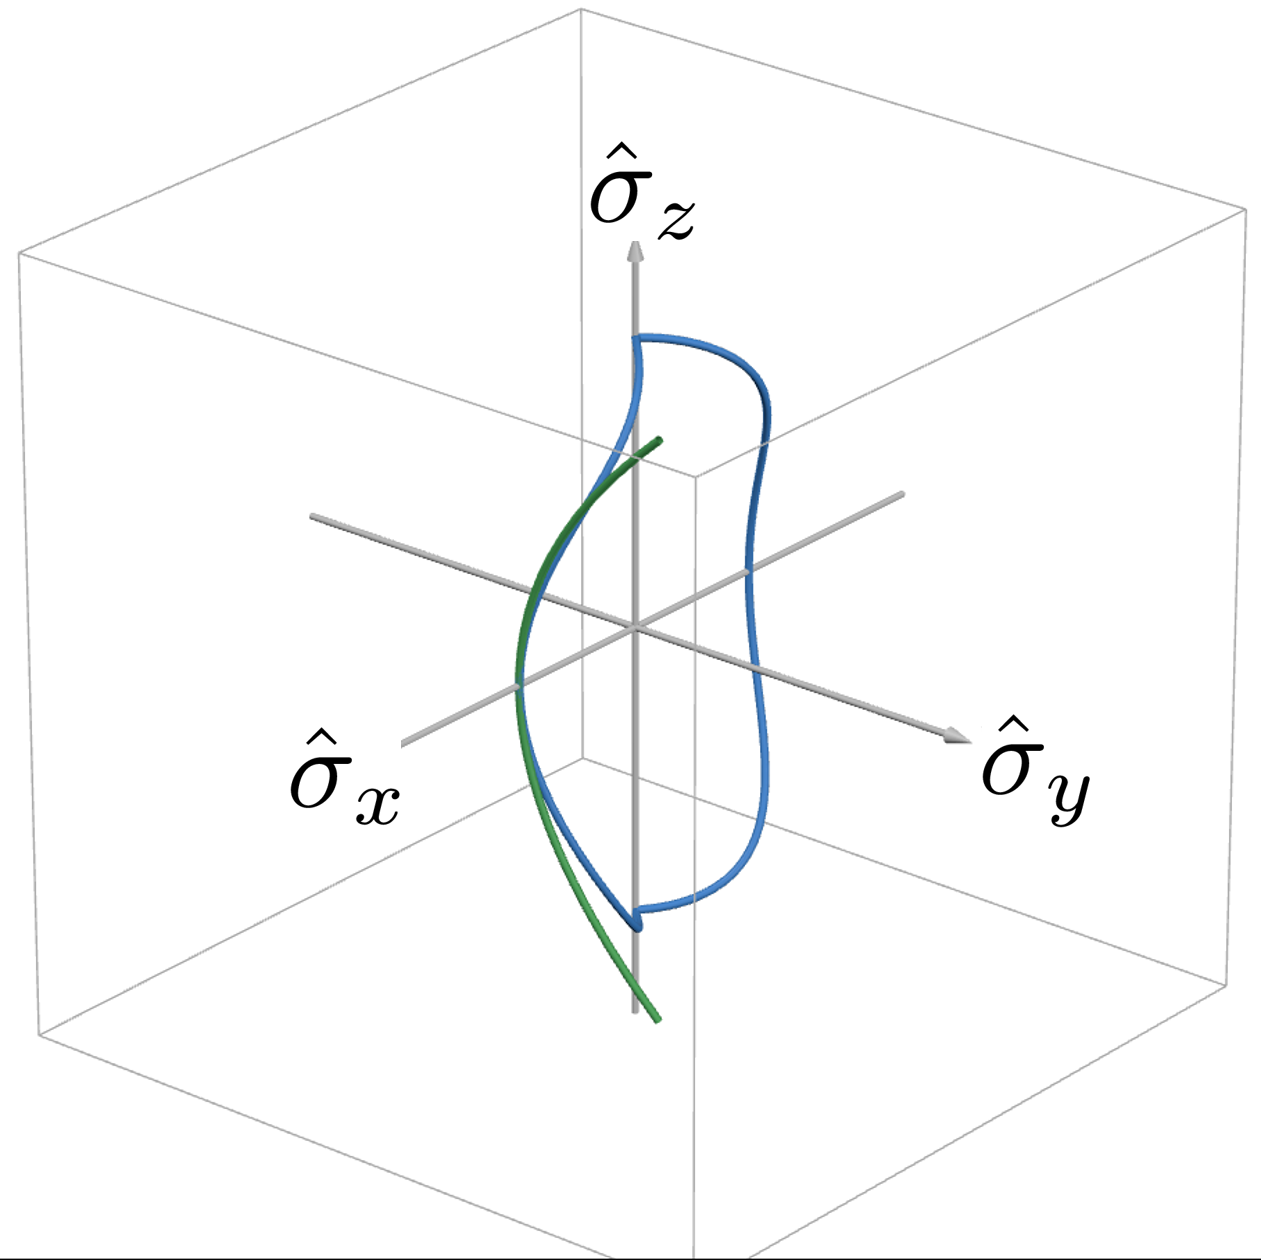
\includegraphics[scale=0.5]{figures/TLZ_CE2_1.png}
  \caption{TLZモデルを含むcyclic evolutionで整流作用を取り入れない系(\ref{TLZ_CE_2})におけるHamiltonianの経路}
  \label{fig:TLZ_CE2_1}
\end{figure}

\begin{figure}[htbp]
  \centering
  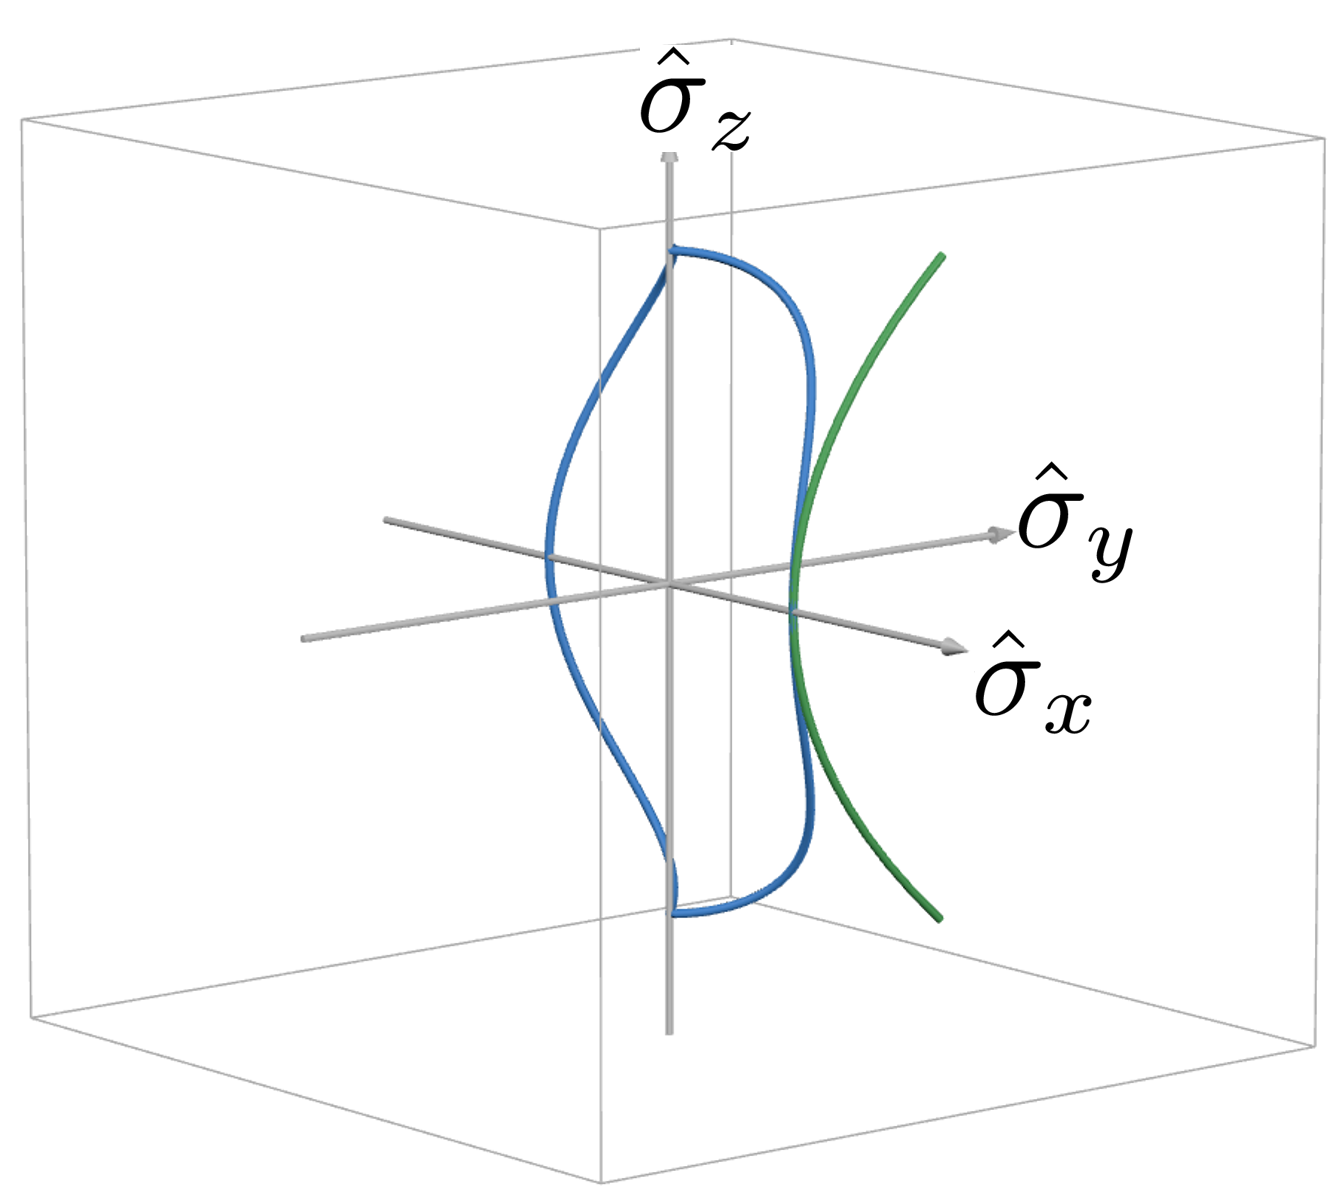
\includegraphics[scale=0.5]{figures/TLZ_CE2_2.png}
  \caption{TLZモデルを含むcyclic evolutionで整流作用を取り入れない系(\ref{TLZ_CE_2})におけるHamiltonianの経路(別の角度からの視点)}
  \label{fig:TLZ_CE2_2}
\end{figure}

\begin{figure}[htbp]
  \centering
  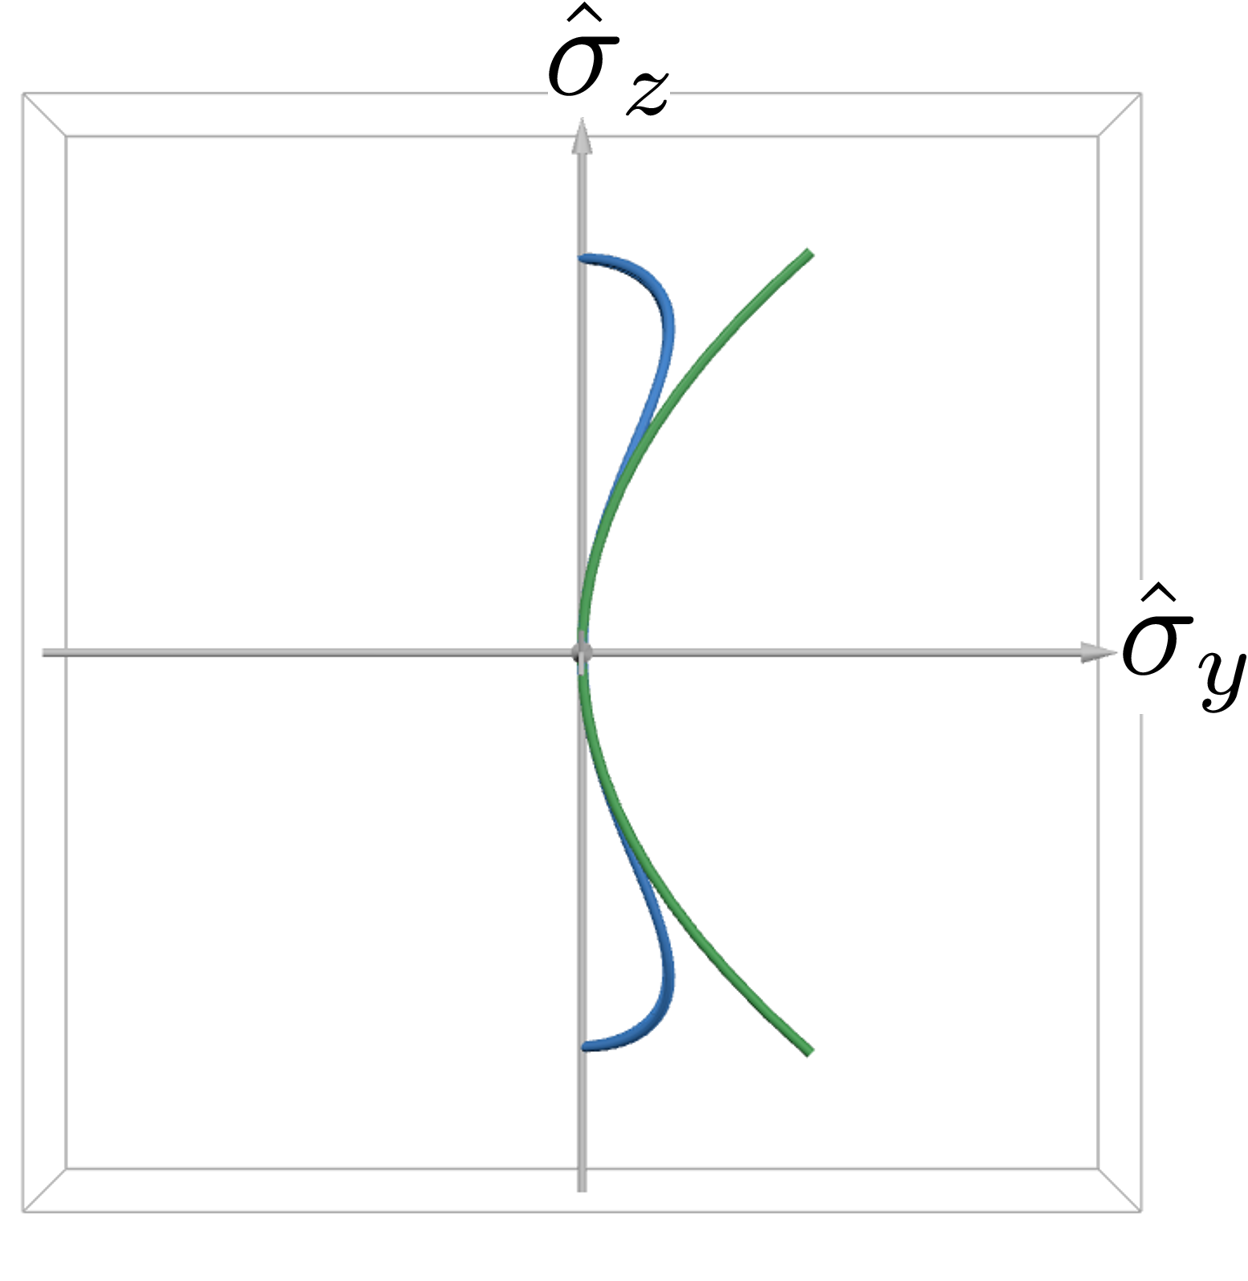
\includegraphics[scale=0.5]{figures/TLZ_CE2_3.png}
  \caption{TLZモデルを含むcyclic evolutionで整流作用を取り入れない系(\ref{TLZ_CE_2})におけるHamiltonianの経路($x$軸視点)}
  \label{fig:TLZ_CE2_3}
\end{figure}

\begin{figure}[htbp]
  \centering
  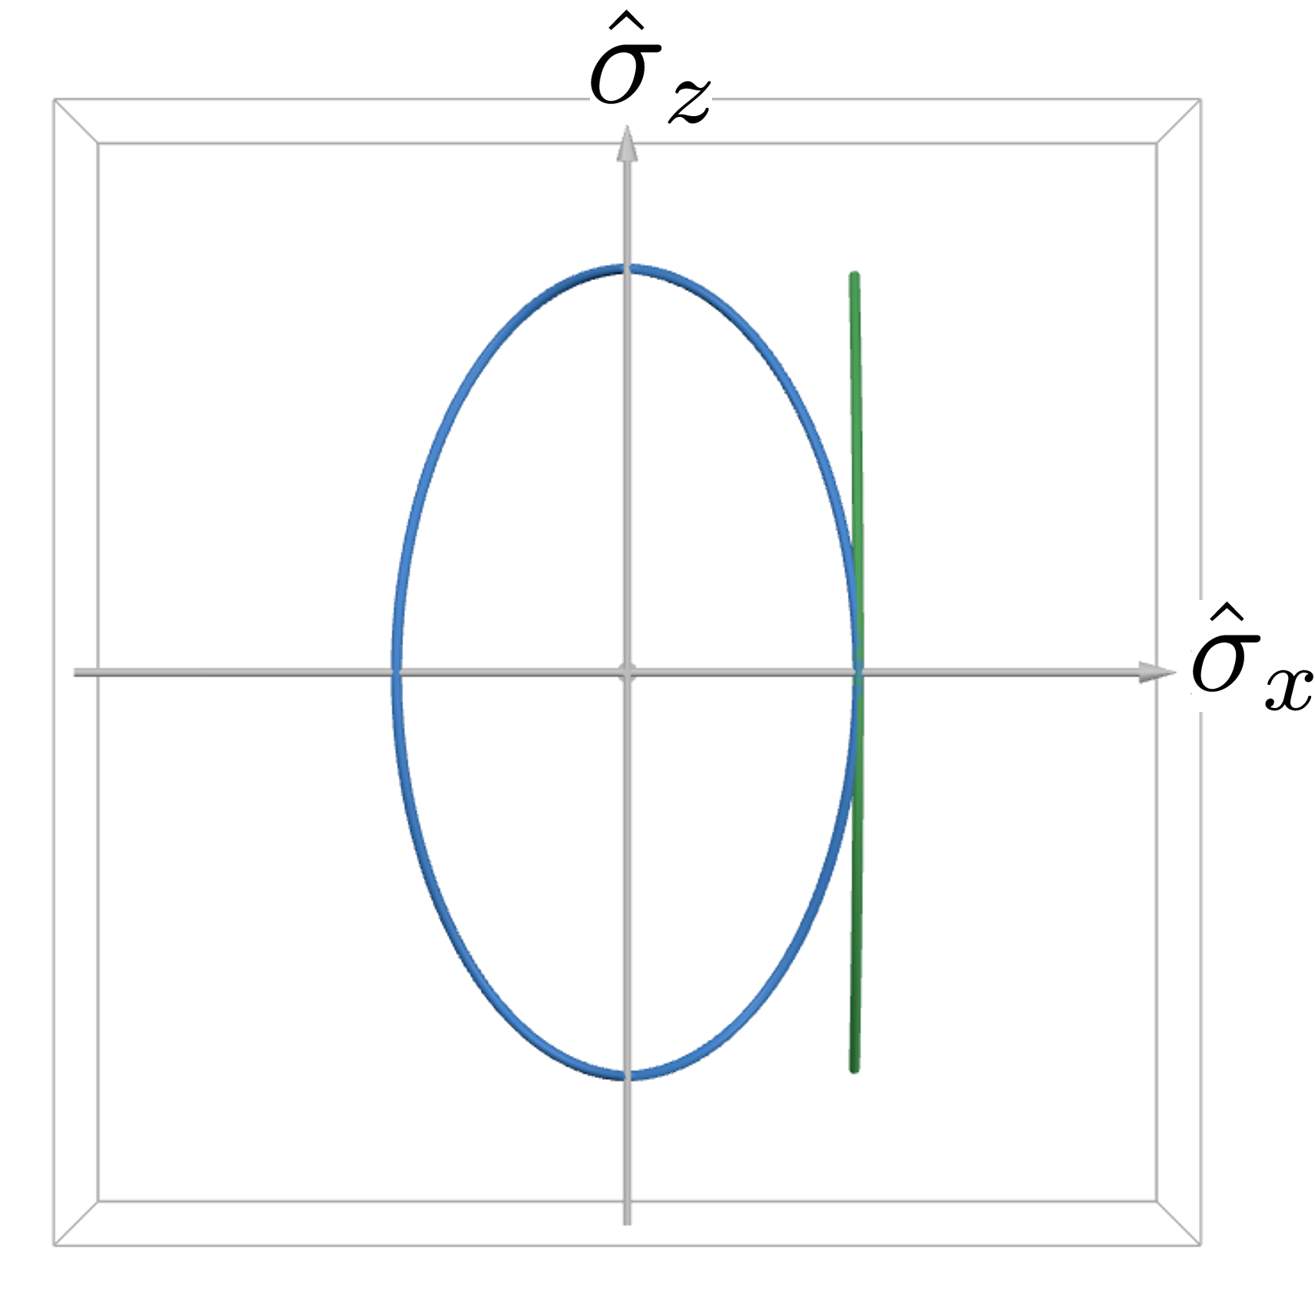
\includegraphics[scale=0.5]{figures/TLZ_CE2_4.png}
  \caption{TLZモデルを含むcyclic evolutionで整流作用を取り入れない系(\ref{TLZ_CE_2})におけるHamiltonianの経路($y$軸視点)}
  \label{fig:TLZ_CE2_4}
\end{figure}

\begin{figure}[htbp]
  \centering
  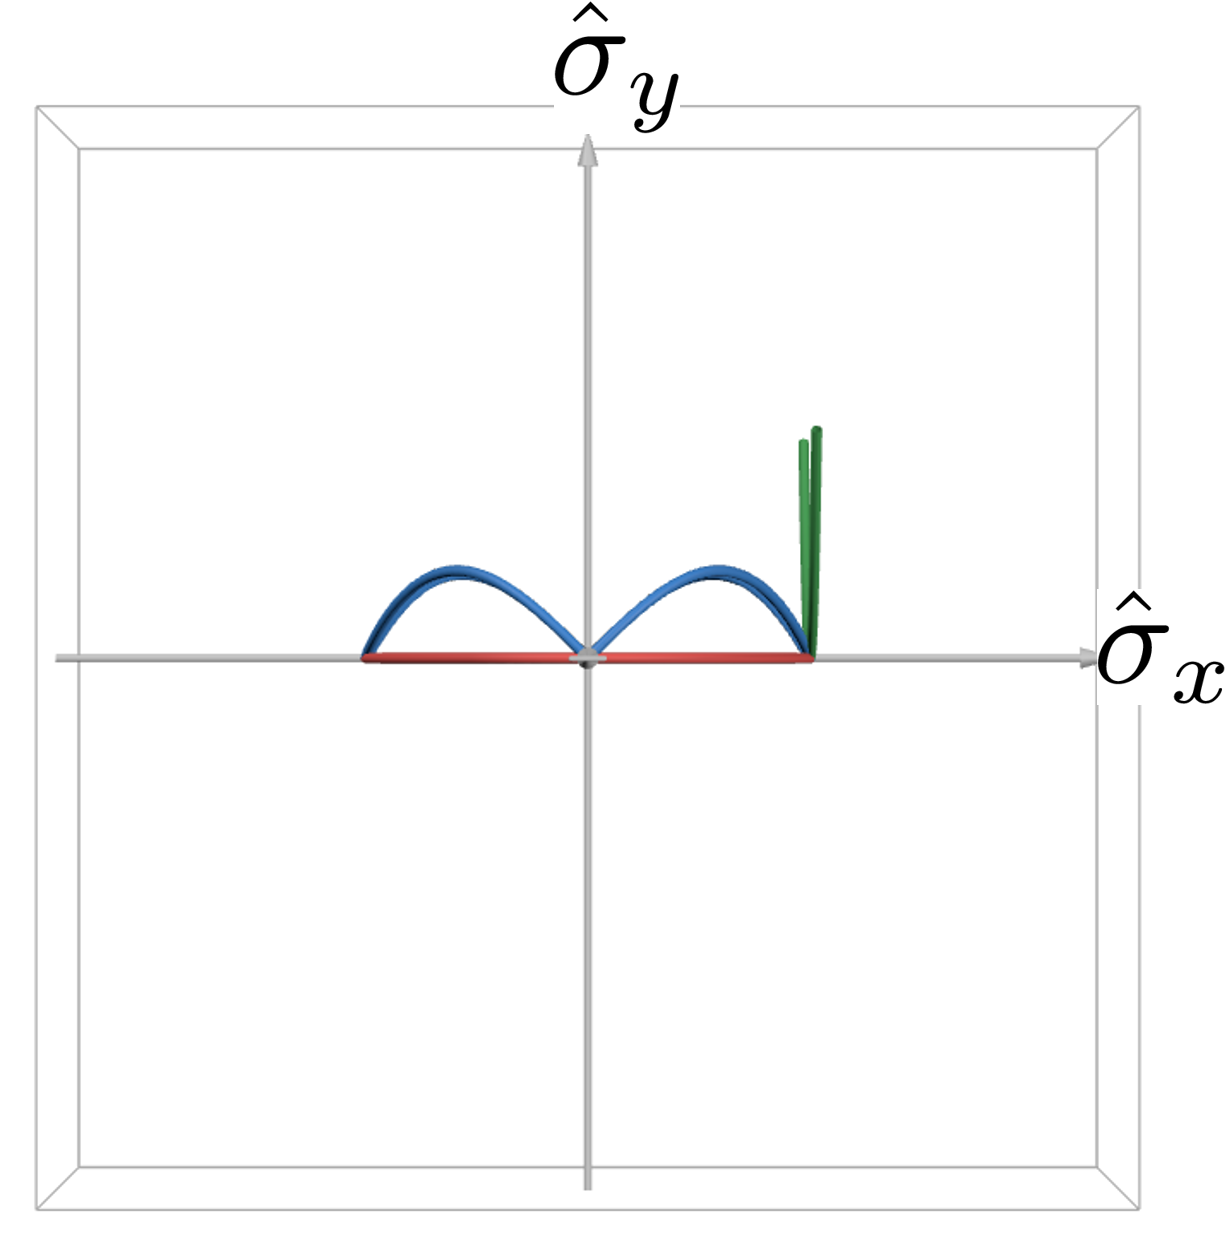
\includegraphics[scale=0.5]{figures/TLZ_CE2_5.png}
  \caption{TLZモデルを含むcyclic evolutionで整流作用を取り入れない系(\ref{TLZ_CE_2})におけるHamiltonianの経路($z$視点)}
  \label{fig:TLZ_CE2_5}
\end{figure}

\begin{figure}[htbp]
  \centering
  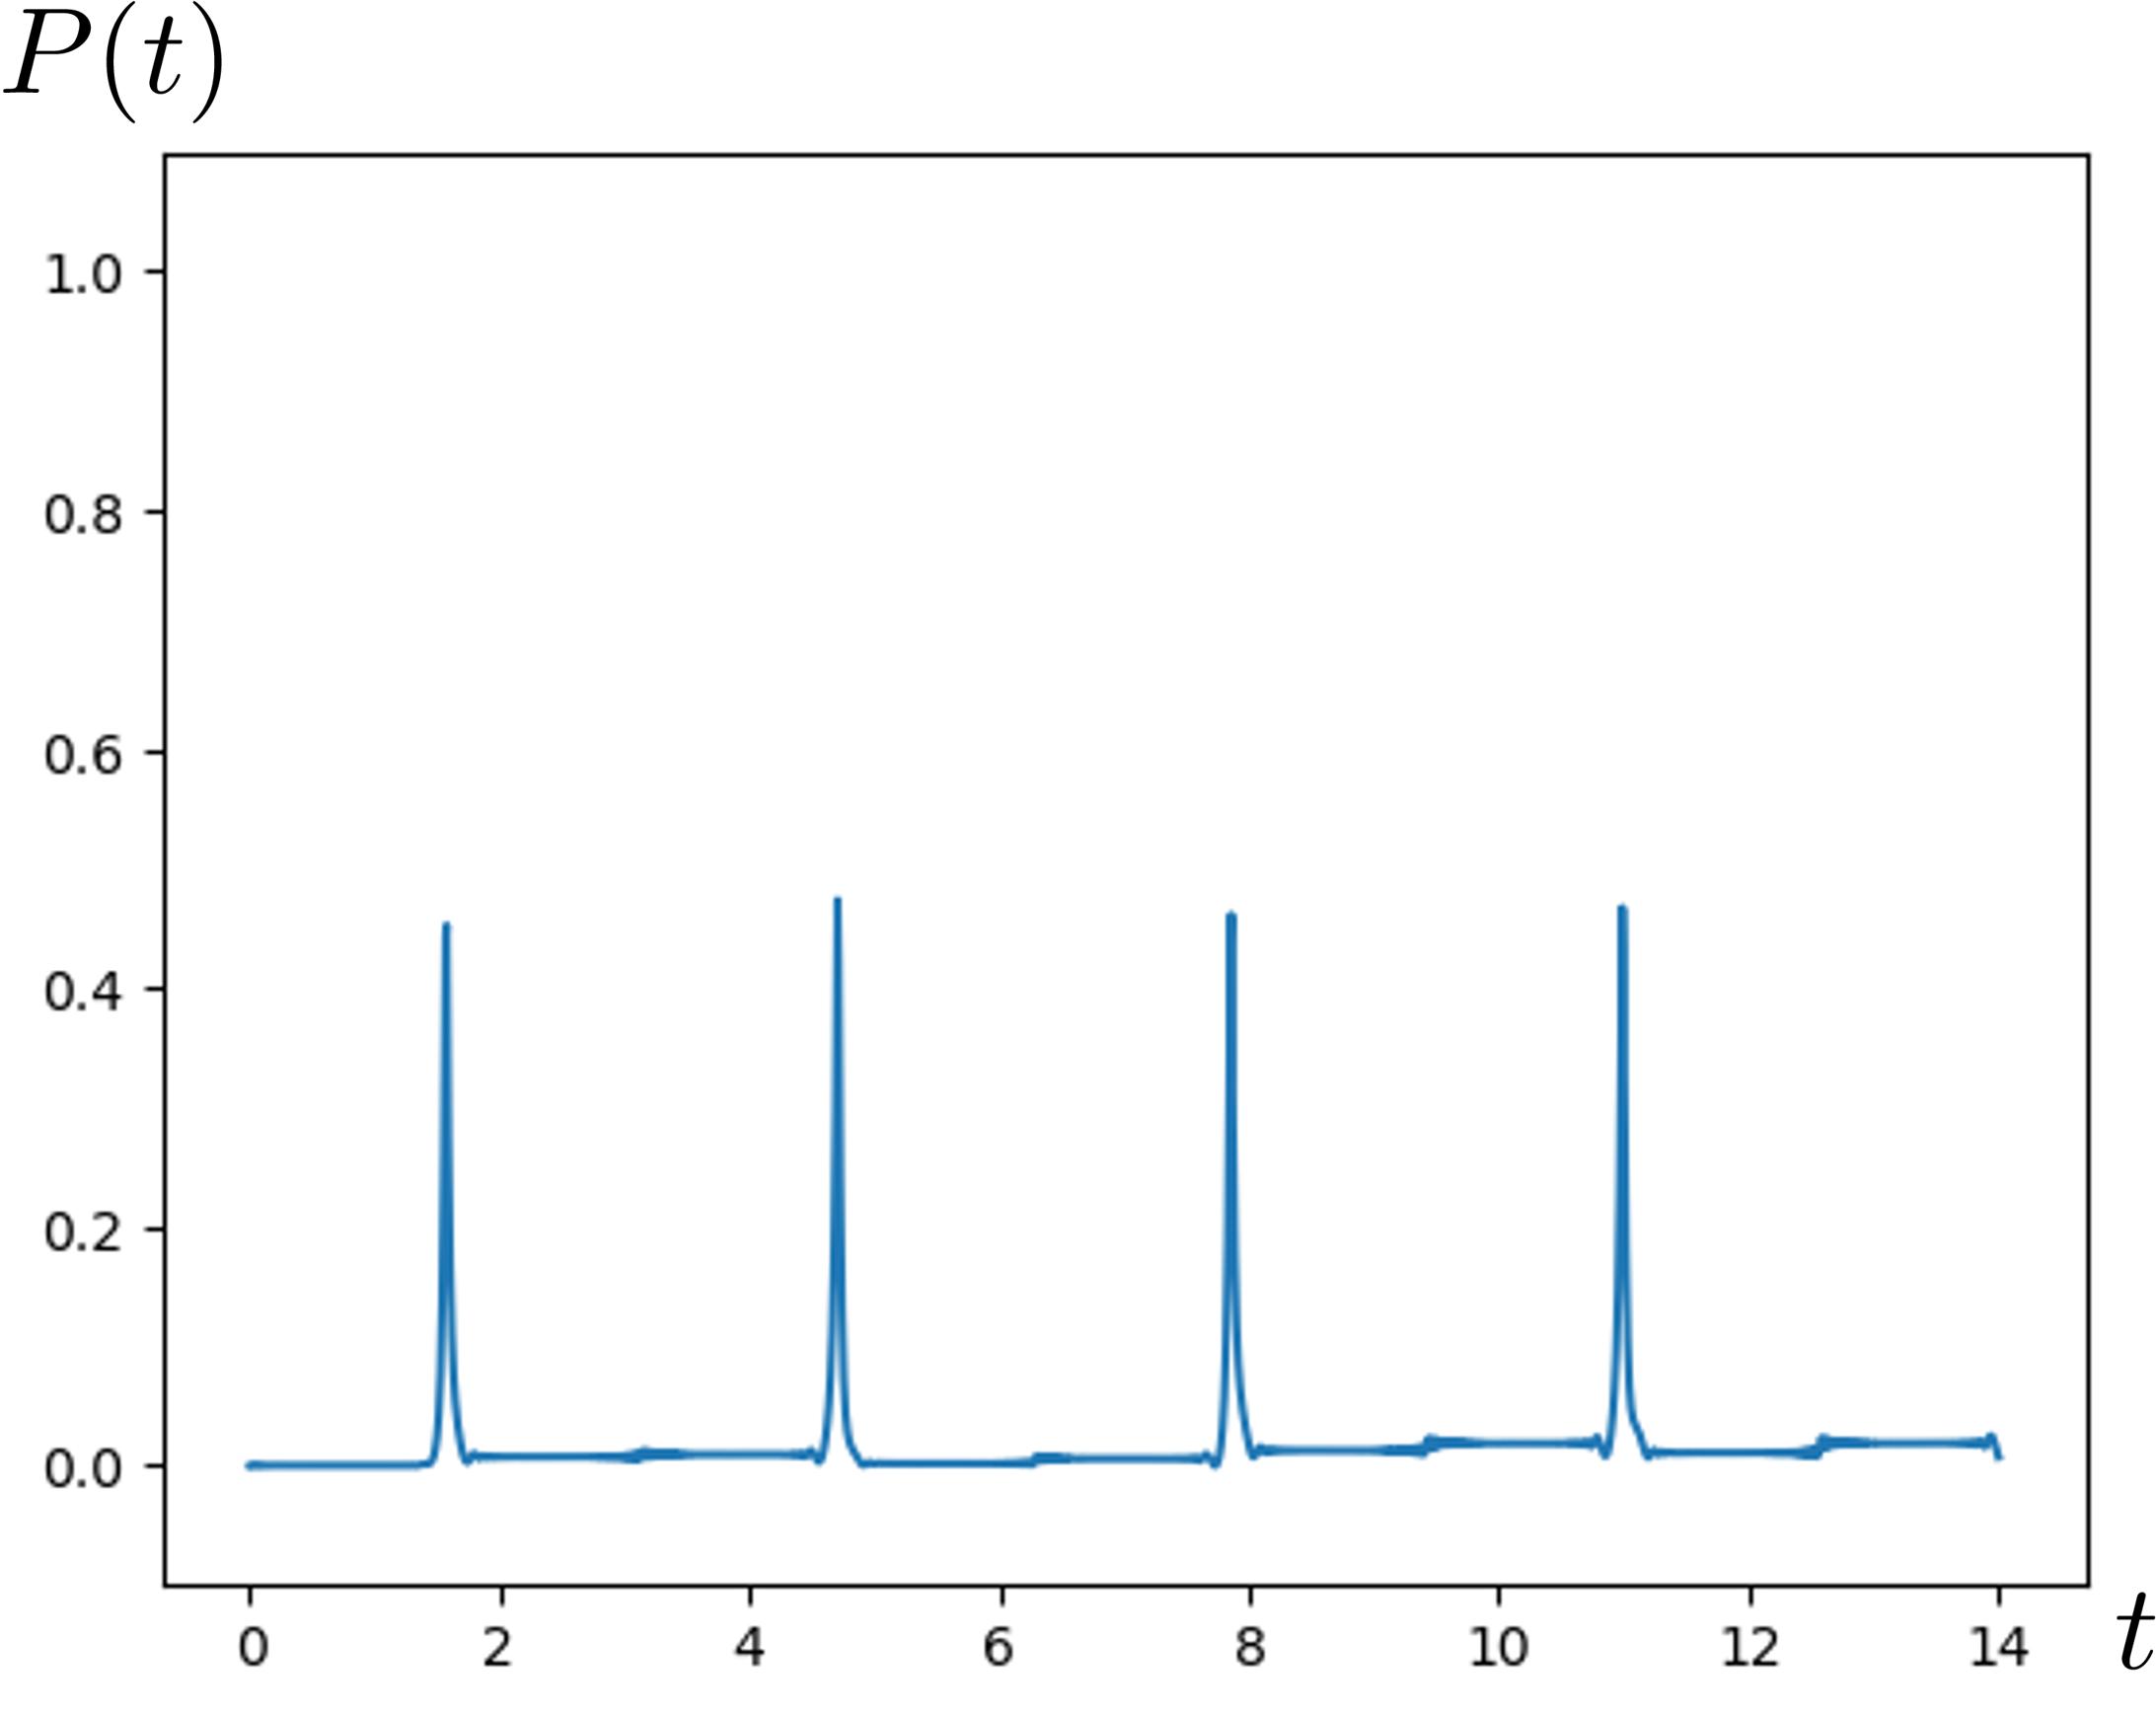
\includegraphics[scale=0.5]{figures/TLZ_CE_perfect.png}
  \caption{$\kappa_g = 0.27$のとき,TLZ遷移を含むcyclic evolutionで整流作用を取り入れない系(\ref{TLZ_CE_2})が,状態$|1\rangle$である確率.$\varepsilon_0=90, \Delta_0 = 3, \omega=1$とした.}
  \label{fig:TLZ_CE_perfect}
\end{figure}